% !TEX encoding = UTF-8
% !TEX program = pdflatex
% !TEX root = AALP.tex
% !TEX spellcheck = it-IT

% 11 Ottobre 2016
% Section Sintassi del linguaggio
% Subsection Sostituzione

\section{Semantica operazionale}

Useremo la semantica operazionale small-step la quale descrive i passi di esecuzione del programma in termini di una relazione di transizione $M \rightarrow M'$.
Questi termini $M$ possono essere visti come gli stati di una macchina astratta.

Un \textbf{valore} rappresenta uno stato finale della macchina astratta e tipicamente sono un sotto insieme di termini. Come notazione usiamo $v$ al posto di $M$.

Nel nostro linguaggi i valori sono:

$$
v = \text{true} \: | \: \text{false} \:|\: n \: | \: \text{fn }x.M
$$

\subsection{Assiomi e regole della semantica}

\begin{figure}[htpb]
	\centering
	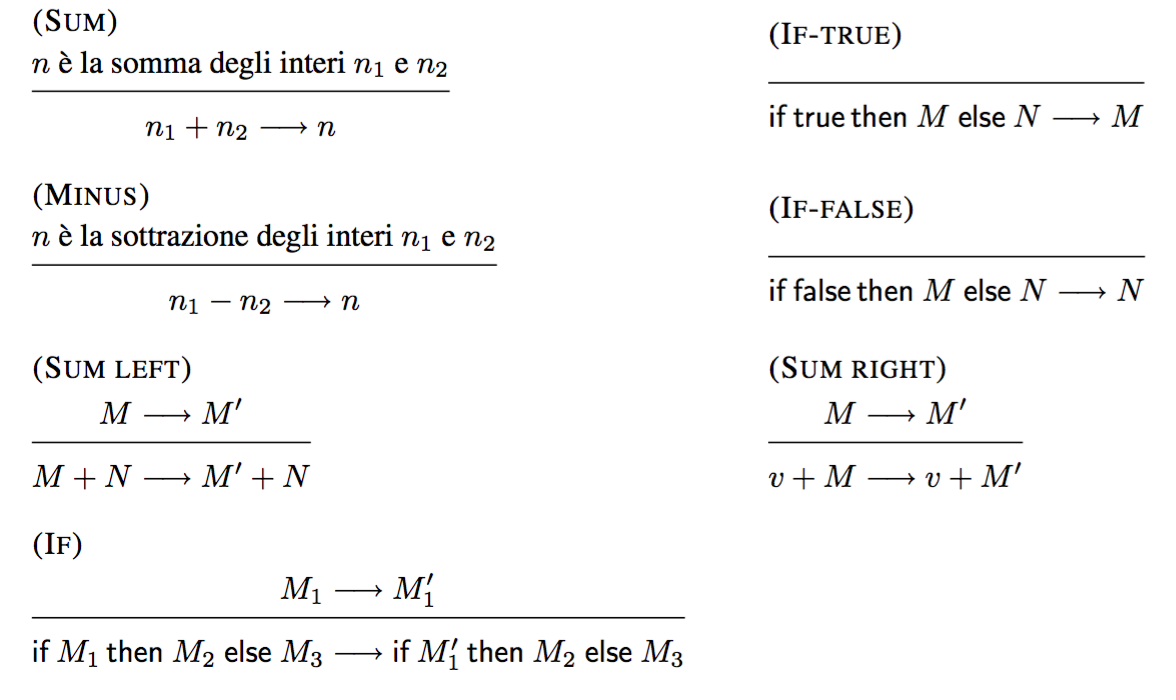
\includegraphics[width = 0.7\linewidth]{./images/l3-assiomi}
	\caption{Assiomi e regole della nostra semantica operazionale}
\end{figure}

\textsc{Sum}, \textsc{Minus}, ecc. sono assiomi che descrivono come avanza la computazione.

\textsc{Sum-Left} e \textsc{Sum-Right} sono delle \textbf{regole} e vengono lette come ``se $M \rightarrow M'$ allora anche il termine più complesso $M + N$ fa un passo in avanti e va su $M' + N$ ($M + N \rightarrow M' +N$). Esiste anche la versione duale \textsc{Minus-Left} e \textsc{Minus-Right}.

Questo insieme di assiomi e regole fornisce una strategia di valutazione per le operazioni del programma, che per come è definita segue un approccio \textit{eager} \todo{Eager? ascoltare registrazione} in quanto vengono valutati solamente i termini necessari alla computazione.

Consideriamo il programma 

$$
\iif \true \then 3+2 \eelse 6+1
$$

\noindent per l'assioma \textsc{If-True} il programma fa un passo di computazione:

$$
\iif \true \then 3+2 \eelse 6+1 \rightarrow 3+2
$$

\noindent e per l'assioma \textsc{Sum} c'è un altro passo da fare

$$
3+2 \rightarrow 5
$$

\noindent così facendo si ottiene il valore che viene calcolato dal programma.

Nell'esempio precedente il termine contenuto nel ramo \text{else} dell'\text{if} non viene valutato.

\textbf{N.B.}: I termini \textit{eager} e \textit{lazy} vengono per qualche strano motivo utilizzati al contrario, stando alla Crafa hanno un significato ambiguo. Meglio non usarli.

\subsection{Applicazione di una funzione - call-by-value e call-by-name}

\begin{figure}[htpb]
	\centering
	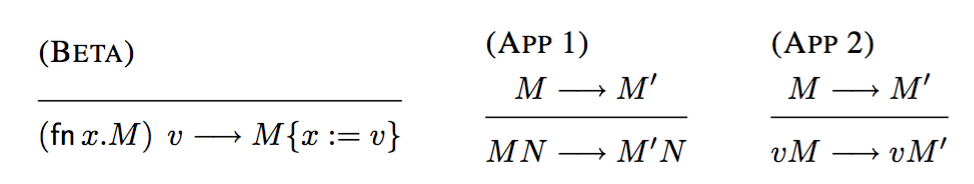
\includegraphics[width = 0.7\linewidth]{./images/l3-assiomi-2}
	\caption{Assiomi e regole per l'applicazione di una funzione}
\end{figure}

\noindent Questo stile di gestire l'applicazione di una funzione prende il nome di \textbf{call-by-value} e viene determinata dall'assioma \textsc{Beta}, perché l'argomento viene valutato prima di essere applicato alla funzione.
Al contrario la sintassi \textbf{call-by-name} permette invece di applicare un termine generico al parametro della funzione.

Le regole di per la sintassi call-by-name la regola \textsc{Beta} diventa

\begin{prooftree}
	\AxiomC{ }
	\LeftLabel{(\textsc{Beta})}
	\UnaryInfC{$\text{fn }x.M \: N \rightarrow M \{ x := N\}$}
\end{prooftree}

\noindent Le regole dell'applicazione cambiano, non è più necessario \textsc{App2} perché serviva per arrivare ad ottenere il valore del parametro.

$$
	M = (\fn x. x+x+x) \: \underbrace{5-(2+1)}_{N}
$$	

\noindent Con la semantica call-by-value è necessario come prima cosa trovare il valore del termine $N$

Per proseguire posso solo applicare \textsc{App2}, perché $M$ è già un valore finale

\begin{prooftree}
	\AxiomC{$5-(2+1) \rightarrow 5 -3$}
	\LeftLabel{\textsc{(App2)}}
	\UnaryInfC{$(\fn x.x+x+x) \:\: 5-(2+1) \rightarrow (\fn x.x+x+x)\: (5-3)$}
\end{prooftree}

\noindent La parte sopra della regola è ancora un'ipotesi, quindi devo continuare a derivare fino a che non dimostro che è vera cercando un assioma, in questo caso serve la regola \textsc{Minus-Right}	

\begin{prooftree}
	\AxiomC{$2+1 \rightarrow 3$}
	\LeftLabel{\textsc{(Minus-Right)}}
	\UnaryInfC{$5-(2+1) \rightarrow 5 -3$}
	\LeftLabel{\textsc{(App2)}}
	\UnaryInfC{$(\fn x.x+x+x) \: \: 5-(2+1) \rightarrow (\fn x.x+x+x)\: (5-3)$}
\end{prooftree}


\noindent allo stesso modo devo applicare l'assioma \textsc{Sum} per l'ipotesi $2+1\rightarrow3$

\begin{prooftree}
	\AxiomC{$\checkmark$}
	\LeftLabel{\textsc{Sum}}
	\UnaryInfC{$2+1 \rightarrow 3$}
	\LeftLabel{\textsc{(Minus-Right)}}
	\UnaryInfC{$5-(2+1) \rightarrow 5 -3$}
	\LeftLabel{\textsc{(App2)}}
	\UnaryInfC{$(\fn x.x+x+x) \: \: 5-(2+1) \rightarrow (\fn x.x+x+x)\: (5-3)$}
\end{prooftree}

\noindent Sono quindi arrivato a completare un ramo di derivazione, provando l'ipotesi $(\fn x. x+x+x)\: 5-(2+1) \rightarrow (\fn x.x+x+x)\: (5-3)$, ma non ho ancora finito, perché posso applicare ancora \textsc{App2} dato che non ho ancora ottenuto un valore per il parametro della funzione.

\begin{prooftree}
	\AxiomC{$\checkmark$}
	\LeftLabel{\textsc{(Minus)}}
	\UnaryInfC{$5-3\rightarrow 2$}
	\LeftLabel{\textsc{(App2)}}
	\UnaryInfC{$(\fn x.x+x+x) \: (5-3) \rightarrow (\fn x.x+x+x)\: 2$}
\end{prooftree}

\noindent Adesso posso applicare l'assioma \textsc{Beta}:

\begin{prooftree}
	\AxiomC{}
	\LeftLabel{\textsc{(Beta)}}
	\UnaryInfC{$(\fn x.x+x+x)\: 2 \rightarrow 2+(2+2)$}
\end{prooftree}

\noindent e da li posso continuare con

\begin{prooftree}
	\AxiomC{$\checkmark$}
	\LeftLabel{\textsc{(Sum)}}
	\UnaryInfC{$2+2\rightarrow 4$}
	\LeftLabel{\textsc{(Sum-Right)}}
	\UnaryInfC{$2+(2+2) \rightarrow 2+4$}
\end{prooftree}

\noindent e poi concludo con

\begin{prooftree}
	\AxiomC{$\checkmark$}
	\LeftLabel{\textsc{(Sum)}}
	\UnaryInfC{$2+4\rightarrow 6$}
\end{prooftree}

\noindent quindi con call-by-value si arriva al valore 6 con 5 passi.

Utilizzando call-by-name si ottiene sempre lo stesso risultato, con la differenza che viene applicata prima la regola \textsc{Beta} che porta ad avere

$$
M \rightarrow (5-(2+1)) + [(5-(2+1)) + (5-(2+1))]
$$

\noindent per esercizio continuare l'albero di derivazione. \todo{TODO}

\vspace{10px}

Consideriamo il termine $M = (\fn x.x+x+x)\: N $ con 100 passi necessari per arrivare al valore di $N$.
In questo caso utilizzando call-by-name è necessario effettuare 3 volte il calcolo del valore di $N$, perché il valore del parametro $x$ viene usato 3 volte, mentre con la sintassi call-by-value la valutazione di $N$ viene effettuata una sola volta. Questa differenza non è sempre presente.

Consideriamo invece il programma $M' = (\fn x.3+5) \:N$ con lo stesso $N$ di prima. Si ha che è più efficiente il call-by-name perché il valore di $N$ non viene utilizzato all'interno della funzione e quindi non viene calcolato, mentre con call-by-value il valore di $N$ viene calcolato.

Casi estremi a parte, si è visto che mediamente è più conveniente utilizzare call-by-value.

Un altro programma interessante è $\Omega = (\fn x.x \: x)\: (\fn x. x\:x)$ sia con call-by-value che call-by-n ottengo $(\fn x.x x)\: (\fn x.x x)$, ovvero ottengo ancora $\Omega$.
La semantica di questo programma è divergente, perché l'esecuzione di un passo di computazione porta esattamente alla stessa situazione.
Un'altra cosa interessante di questo esempio è che il parametro viene applicato a se stesso e quindi risulta impossibile trovare un tipo per questo parametro, perché dovrebbe essere sempre un tipo di ordine superiore di se stesso.

\subsection{Errori semantici}
$M = 5 + \text{false}$ è un programma sintatticamente corretto, ma che non riesco a far avanzare perché non ho nessun assioma o regola che posso applicare, quindi da $M$ non riesco a passare ad un $M'$. Inoltre $M$ non è neanche un valore finale.
In questo caso si ha quindi un'errore di programmazione e il termine $M$ prende il nome di termine \textbf{stuck}.


$$M = (\fn x.\iif x \text{ then true else false})\: (\text{if false then fn }y.\text{ true else } 4)$$

\noindent L'unica regola che posso applicare è \textsc{App2}, perché la prima parte del termine è già un valore.

$$(\fn x.\iif x \text{ then true else false}) \:(\text{if false then fn }y.\text{ true else } 4) \rightarrow (\fn x.\iif x \text{ then true else false})\: 4$$

\noindent Adesso posso applicare \textsc{Beta}:

$$(\fn x.\iif x \text{ then true else false})\: 4 \rightarrow \iif 4 \text{ then true else false}$$

\noindent ottenendo un termine stuck perché la guardia dell'\text{if} non è booleana.

\subsection{Deterministicità del linguaggio}

La semantica del linguaggio è \textbf{deterministica}, ovvero per ogni stato c'è al più un solo passo che posso eseguire.

Più formalmente se $M \rightarrow M'$ e $M \rightarrow M''$ allora $M' = M''$.

Questo si dimostra per induzione sulla struttura di $M$ (vedi §\ref{ex:2.1.4}). 

\subsection{Scala: call-by-name e call-by-value}

In Scala è possibile andare a scegliere se utilizzare il passaggio di parametri con call-by-name o call-by-value.

Questo può portare ad un problema a livello pratico, ad esempio se si vuole implementare un meccanismo di asserzioni che può essere disabilitato, ci possono essere dei problemi.

\begin{lstlisting}[language=Scala]
	var assEnabled = true
	def assert(pred: Boolean) = 
		if (assEnabled && !pred)
			throw new AssException
	...
	assert(saldoConto() > 0)
\end{lstlisting}

\noindent Un po' di informazioni su Scala:
\begin{itemize}
	\item In Scala un valore che può essere modificato viene identificato con \texttt{var}.
	\item Non è necessario specificare il tipo di ritorno di una funzione.
	\item Se la funzione è composta da una sola espressione non serve il \texttt{return}.
\end{itemize}

\noindent Tornando all'esempio, assumendo di aver disabilitato le asserzioni impostando il flag a \texttt{false} si ha che che con il call-by-value la funzione \texttt{saldoConto()} viene comunque valutata.

Utilizzando invece call-by-name, la funzione \texttt{saldoConto()} viene calcolata solo se le asserzioni sono abilitate.

Per specificare che un parametro deve essere passato by-name è necessario specificarlo nel tipo del parametro:

\begin{center}
\texttt{pred : =>Boolean}
\end{center}